\documentclass[a4]{article}
\pagestyle{myheadings}

%%%%%%%%%%%%%%%%%%%
% Packages/Macros %
%%%%%%%%%%%%%%%%%%%
\usepackage{mathrsfs}


\usepackage{fancyhdr}
\pagestyle{fancy}
\lhead{}
\chead{}
\rhead{}
\lfoot{}
\cfoot{} 
\rfoot{\normalsize\thepage}
\renewcommand{\headrulewidth}{0pt}
\renewcommand{\footrulewidth}{0pt}
\newcommand{\RomanNumeralCaps}[1]
    {\MakeUppercase{\romannumeral #1}}

\usepackage{amssymb,latexsym}  % Standard packages
\usepackage[utf8]{inputenc}
\usepackage[russian]{babel}
\usepackage{MnSymbol}
\usepackage{mathrsfs}
\usepackage{amsmath,amsthm}
\usepackage{indentfirst}
\usepackage{graphicx}%,vmargin}
\usepackage{graphicx}
\graphicspath{{pictures/}} 
\usepackage{verbatim}
\usepackage{color}
\usepackage{color,colortbl}
\usepackage[nottoc,numbib]{tocbibind}
\usepackage{float}
\usepackage{multirow}
\usepackage{hhline}

\usepackage{listings}
\definecolor{codegreen}{rgb}{0,0.6,0}
\definecolor{codegray}{rgb}{1,1,1}
\definecolor{codepurple}{rgb}{0.58,0,0.82}
\definecolor{backcolour}{rgb}{0.95,0.95,0.92}
 
\lstdefinestyle{mystyle}{
    backgroundcolor=\color{backcolour},   
    commentstyle=\color{codegreen},
    keywordstyle=\color{magenta},
    numberstyle=\tiny\color{codegray},
    stringstyle=\color{codepurple},
    basicstyle=\footnotesize,
    breakatwhitespace=false,         
    breaklines=true,                 
    captionpos=b,                    
    keepspaces=true,                 
    numbers=left,                    
    numbersep=5pt,                  
    showspaces=false,                
    showstringspaces=false,
    showtabs=false,                  
    tabsize=2
}
 
\lstset{style=mystyle}

\usepackage{url}
\urldef\myurl\url{foo%.com}
\def\UrlBreaks{\do\/\do-}
\usepackage{breakurl}
\Urlmuskip=0mu plus 1mu



\DeclareGraphicsExtensions{.pdf,.png,.jpg}% -- настройка картинок

\usepackage{epigraph} %%% to make inspirational quotes.
\usepackage[all]{xy} %for XyPic'a
\usepackage{color} 
\usepackage{amscd} %для коммутативных диграмм
%\usepackage[colorlinks,urlcolor=red]{hyperref}

%\renewcommand{\baselinestretch}{1.5}
%\sloppy
%\usepackage{listings}
%\lstset{numbers=left}
%\setmarginsrb{2cm}{1.5cm}{1cm}{1.5cm}{0pt}{0mm}{0pt}{13mm}


\newtheorem{Lemma}{Лемма}[section]
\newtheorem{Proposition}{Предложение}[section]
\newtheorem{Theorem}{Теорема}[section]
\newtheorem{Corollary}{Следствие}[section]
\newtheorem{Remark}{Замечание}[section]
\newtheorem{Definition}{Определение}[section]
\newtheorem{Designations}{Обозначение}[section]




%%%%%%%%%%%%%%%%%%%%%%% 
%Подготовка оглавления% 
%%%%%%%%%%%%%%%%%%%%%%% 
\usepackage[titles]{tocloft}
\renewcommand{\cftdotsep}{2} %частота точек
\renewcommand\cftsecleader{\cftdotfill{\cftdotsep}}
\renewcommand{\cfttoctitlefont}{\hspace{0.38\textwidth} \LARGE\bfseries} 
\renewcommand{\cftsecaftersnum}{.}
\renewcommand{\cftsubsecaftersnum}{.}
\renewcommand{\cftbeforetoctitleskip}{-1em} 
\renewcommand{\cftaftertoctitle}{\mbox{}\hfill \\ \mbox{}\hfill{\footnotesize Стр.}\vspace{-0.5em}} 
%\renewcommand{\cftchapfont}{\normalsize\bfseries \MakeUppercase{\chaptername} } 
%\renewcommand{\cftsecfont}{\hspace{1pt}} 
\renewcommand{\cftsubsecfont}{\hspace{1pt}} 
%\renewcommand{\cftbeforechapskip}{1em} 
\renewcommand{\cftparskip}{3mm} %определяет величину отступа в оглавлении
\setcounter{tocdepth}{5} 
\renewcommand{\listoffigures}{\begingroup %добавляем номер в список иллюстраций
\tocsection
\tocfile{\listfigurename}{lof}
\endgroup}
\renewcommand{\listoftables}{\begingroup %добавляем номер в список иллюстраций
\tocsection
\tocfile{\listtablename}{lot}
\endgroup}


%\renewcommand{\thelikesection}{(\roman{likesection})}
%%%%%%%%%%%
% Margins %
%%%%%%%%%%%
\addtolength{\textwidth}{0.7in}
\textheight=630pt
\addtolength{\evensidemargin}{-0.4in}
\addtolength{\oddsidemargin}{-0.4in}
\addtolength{\topmargin}{-0.4in}

%%%%%%%%%%%%%%%%%%%%%%%%%%%%%%%%%%%
%%%%%%Переопределение chapter%%%%%% 
%%%%%%%%%%%%%%%%%%%%%%%%%%%%%%%%%%%
\newcommand{\empline}{\mbox{}\newline} 
\newcommand{\likechapterheading}[1]{ 
\begin{center} 
\textbf{\MakeUppercase{#1}} 
\end{center} 
\empline} 

%%%%%%%Запиливание переопределённого chapter в оглавление%%%%%% 
\makeatletter 
\renewcommand{\@dotsep}{2} 
\newcommand{\l@likechapter}[2]{{\bfseries\@dottedtocline{0}{0pt}{0pt}{#1}{#2}}} 
\makeatother 
\newcommand{\likechapter}[1]{ 
\likechapterheading{#1} 
\addcontentsline{toc}{likechapter}{\MakeUppercase{#1}}} 




\usepackage{xcolor}
\usepackage{hyperref}
\definecolor{linkcolor}{HTML}{000000} % цвет ссылок
\definecolor{urlcolor}{HTML}{AA1622} % цвет гиперссылок
 
\hypersetup{pdfstartview=FitH,  linkcolor=linkcolor,urlcolor=urlcolor, colorlinks=true}

%%%%%%%%%%%%
% Document %
%%%%%%%%%%%%

%%%%%%%%%%%%%%%%%%%%%%%%%%%%%
%%%%%%главы -- section*%%%%%%
%%%%section -- subsection%%%%
%subsection -- subsubsection%
%%%%%%%%%%%%%%%%%%%%%%%%%%%%%
\def \newstr {\medskip \par \noindent} 



\begin{document}
\newcolumntype{g}{>{\columncolor{codegray}}c}



\def\contentsname{\LARGE{Содержание}}
\thispagestyle{empty}
\begin{center} 
\vspace{2cm} 
{\Large \sc Санкт-Петербургский Политехнический}\\
\vspace{2mm}
{\Large \sc Университет} им. {\Large\sc Петра Великого}\\
\vspace{1cm}
{\large \sc Институт прикладной математики и механики\\ 
\vspace{0.5mm}
\textsc{}}\\ 
\vspace{0.5mm}
{\large\sc Кафедра прикладной математики}\\
\vspace{15mm}
%\rule[0.5ex]{\linewidth}{2pt}\vspace*{-\baselineskip}\vspace*{3.2pt} 
%\rule[0.5ex]{\linewidth}{1pt}\\[\baselineskip] 
{\huge \sc Курсовая работа \\
\vspace{6mm}
 }
\vspace*{2mm}
%\rule[0.7ex]{\linewidth}{1pt}\vspace*{-\baselineskip}\vspace{3.2pt} 
%\rule[0.5ex]{\linewidth}{2pt}\\ 
\vspace{1cm}

{\sc $3$ курс$,$ группа $3630102/70301$}

\vspace{2cm} 
Студент \hfill Лебедев К.С.\\
\vspace{1cm}
Преподаватель \hfill Баженов А. Н.\\
\vspace{20mm} 

\end{center} 
%\author{Я}
\begin{center}
\vfill {\large\textsc{Санкт-Петербург}}\\ 
2020 г.
\end{center}

%%%%%%%%%%%%%%%%%%%%%%%%%%%%%%%%%%%%%%%%%%%%%%%%%%%%%%%%%%%%%%%%%%%%%%%%%%%%%%%%%%%%%%%%%%%%%%
%\ \\[4cm]

%\rm
%%%%%%%%%%%%%%%%%%%%%%%%%%%%%%%%%%%%%%%%%%%%%%%%%%%%%%%%%%%%%%%%%%%%%%%%%%%%%%%%%%%%%%%%%%%%%%
\newpage
\pagestyle{plain}

%\begin{center}
%\begin{abstract} 

%\end{abstract}

%\end{center}

\newpage
\tableofcontents{}
\newpage
\listoftables{}
\newpage

\section{Постановка задачи}

Для трех выборок $50$, $200$ и $1000$ элементов, сгенерированных согласно закону распределения Фишер c параметрами $\mu = 4$ и $\nu = 2$ и Рэлея с параметром $\sigma = 0.7$ проверить гипотезы о согласии распределения смоделированной выборки с заданным законом распределения по критерию $\chi^2$ для группирования выбирать интервалы равной длины, уровень значимости $\alpha = 0.05$. Проверить гипотезы о согласии распределения смоделированной выборки с заданным законом распределения по непараметрическому критерию Мизеса-Смирнова; уровень значимости $\alpha = 0.05$. 

\section{Реализация}
Работы была выполнена на языке $Python 3.7.$
Для генерации выборок использовался модуль \cite{numpy}.
Для построения графиков использовалась библиотека matplotlib \cite{plotlib}.
Функции распределения обрабатывались при помощи библиотеки scipy.stats \cite{skp}

\section{Результаты}
\subsection{функция распределения Фишер}
\begin{center}

\begin{figure}[H]
\caption{Функция распределения Фишер с $ n = 50$}
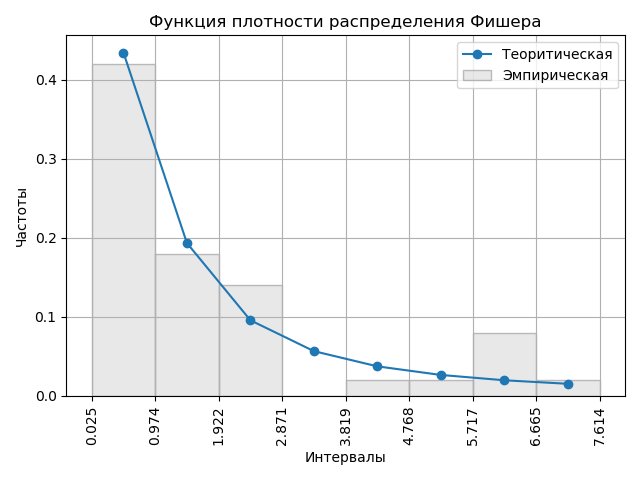
\includegraphics[width=\textwidth]{output/task1/fisher_50_histogram.png}
\end{figure}

\begin{figure}[H]
\caption{Функция нормального распределения с $ n = 50$}
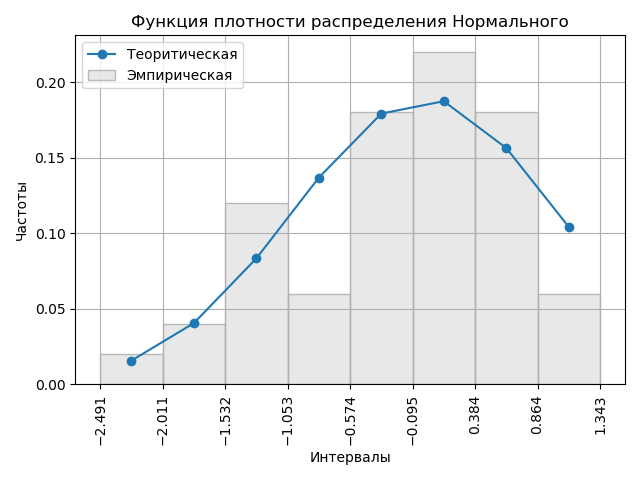
\includegraphics[width=\textwidth]{output/task1/norm_50_histogram.png}
\end{figure}

\begin{figure}[H]
\caption{Функция распределения Фишер с $ n = 200$}
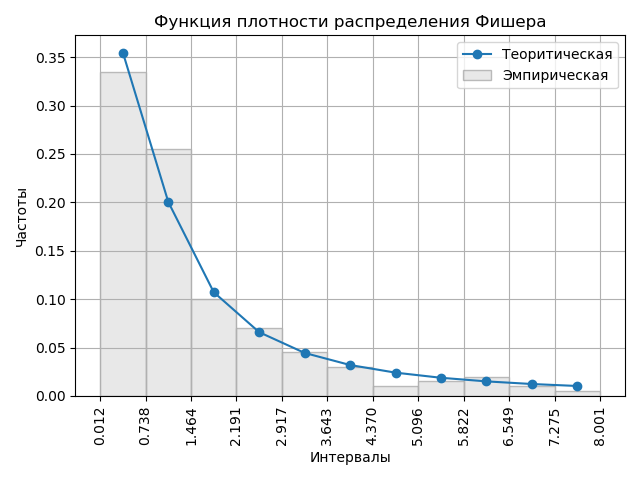
\includegraphics[width=\textwidth]{output/task1/fisher_200_histogram.png}
\end{figure}

\begin{figure}[H]
\caption{Функция нормального распределения с $ n = 200$}
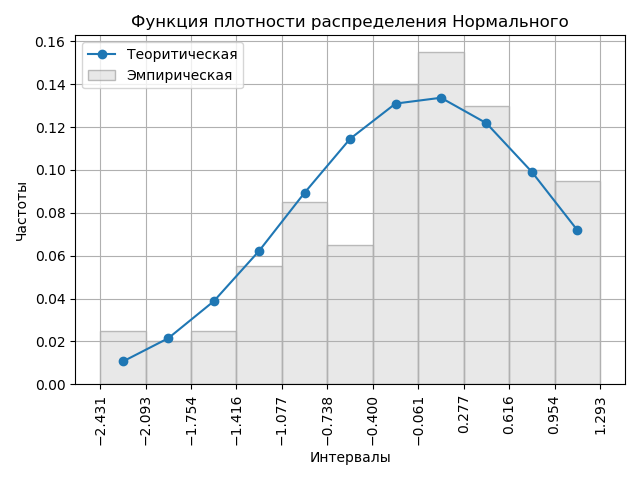
\includegraphics[width=\textwidth]{output/task1/norm_200_histogram.png}
\end{figure}

\begin{figure}[H]
\caption{Функция распределения Фишер с $ n = 1000$}
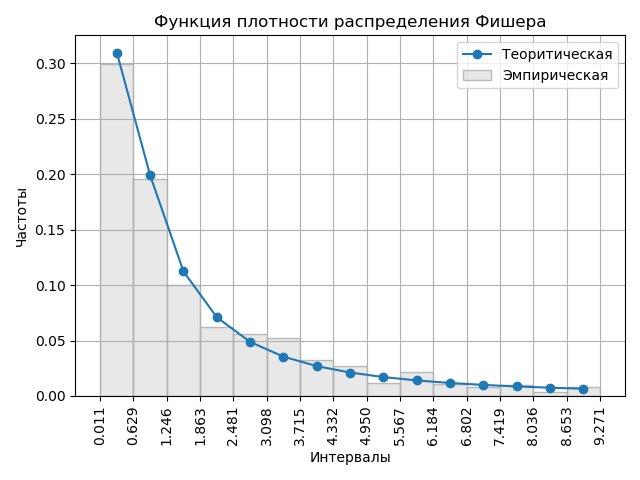
\includegraphics[width=\textwidth]{output/task1/fisher_1000_histogram.png}
\end{figure}

\begin{figure}[H]
\caption{Функция нормального распределения с $ n = 1000$}
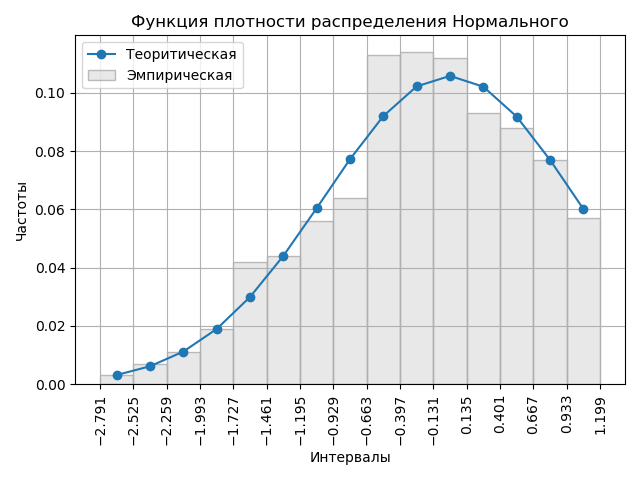
\includegraphics[width=\textwidth]{output/task1/norm_1000_histogram.png}
\end{figure}

\begin{figure}[H]
\caption{График функции распределения Фишер}
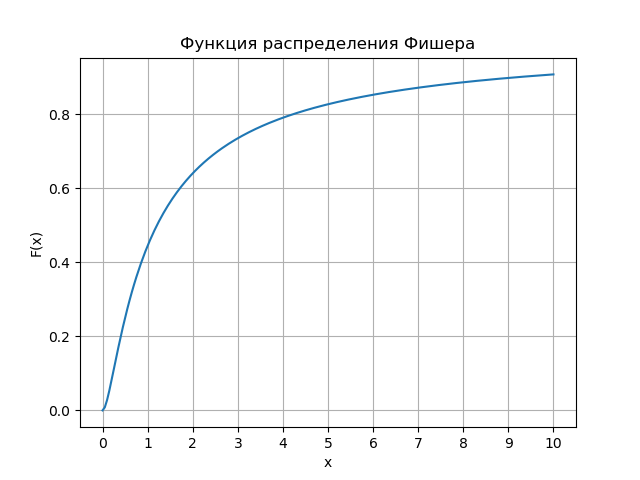
\includegraphics[width=\textwidth]{output/task1/fisher_chart.png}
\end{figure}

\begin{figure}[H]
\caption{График функции нормального распределения}
\includegraphics[width=\textwidth]{output/task1/norm_chart.png}
\end{figure}

\end{center}

\subsection{функция распределения Рэлея}
\begin{center}

\begin{figure}[H]
\caption{Функция распределения Рэлея с $ n = 50$}
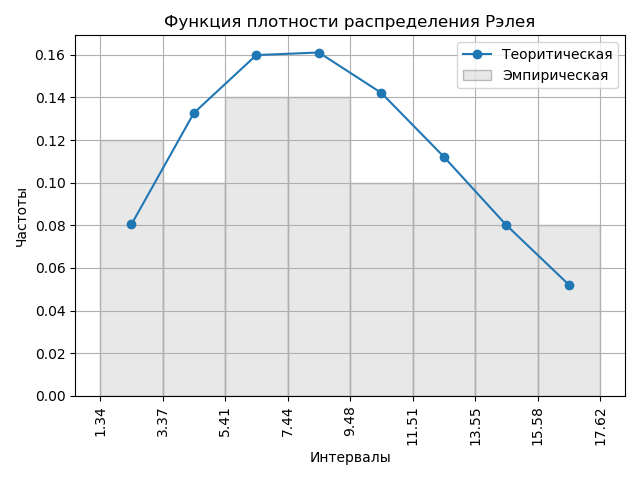
\includegraphics[width=\textwidth]{output/task2/rayleigh_50_histogram.png}
\end{figure}

\begin{figure}[H]
\caption{Функция нормального распределения с $ n = 50$}
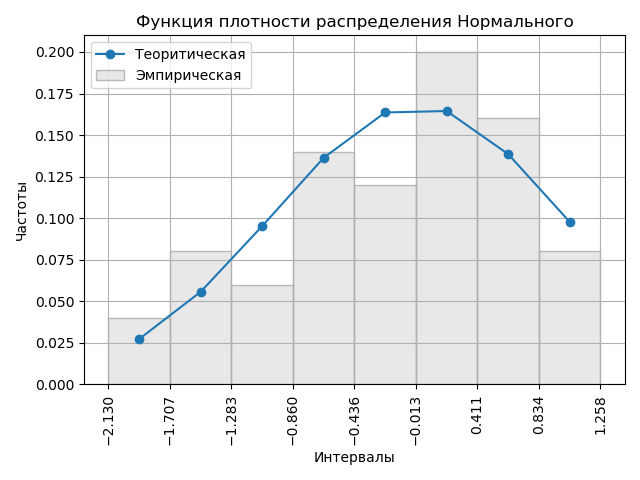
\includegraphics[width=\textwidth]{output/task2/norm_50_histogram.png}
\end{figure}

\begin{figure}[H]
\caption{Функция распределения Рэлея с $ n = 200$}
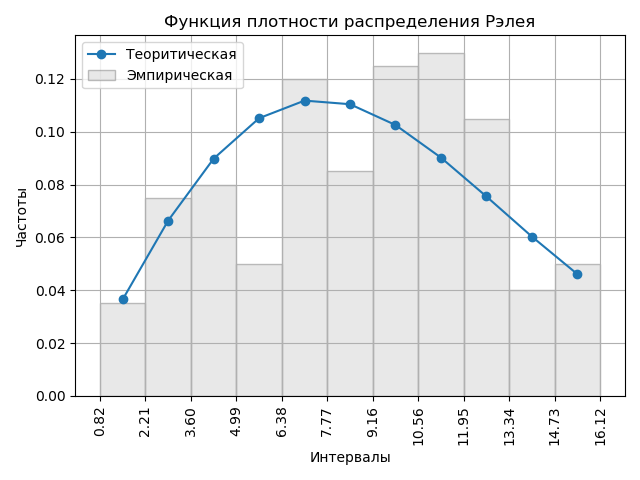
\includegraphics[width=\textwidth]{output/task2/rayleigh_200_histogram.png}
\end{figure}

\begin{figure}[H]
\caption{Функция нормального распределения с $ n = 200$}
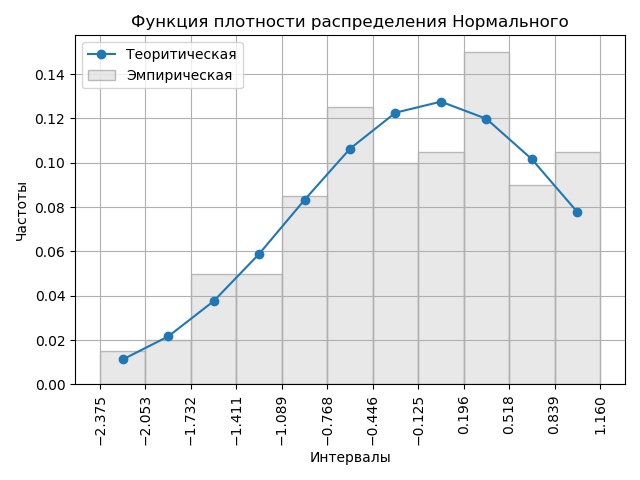
\includegraphics[width=\textwidth]{output/task2/norm_200_histogram.png}
\end{figure}


\begin{figure}[H]
\caption{Функция распределения Рэлея с $ n = 1000$}
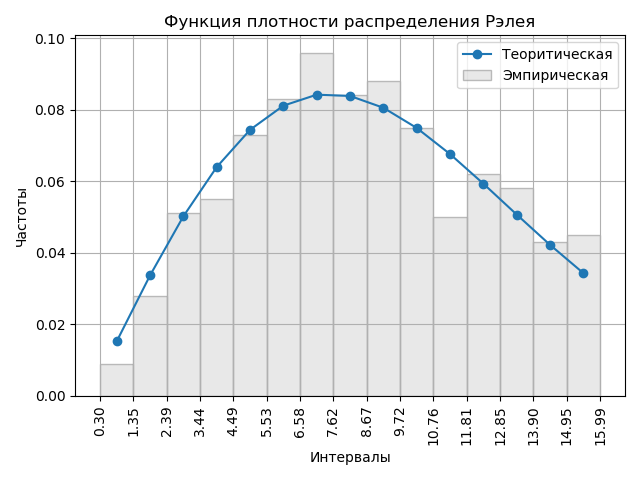
\includegraphics[width=\textwidth]{output/task2/rayleigh_1000_histogram.png}
\end{figure}

\begin{figure}[H]
\caption{Функция нормального распределения с $ n = 1000$}
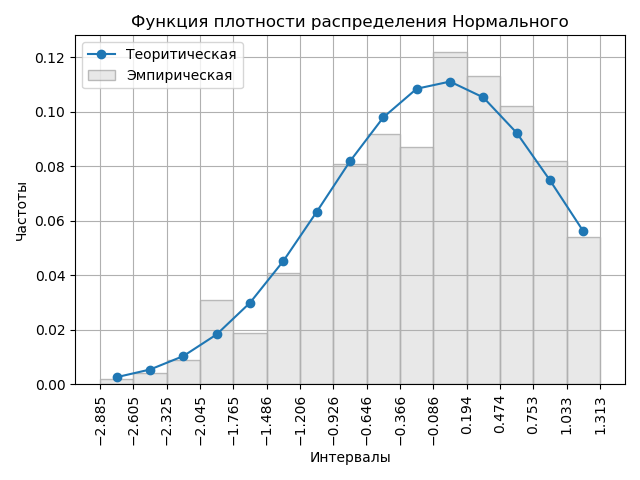
\includegraphics[width=\textwidth]{output/task2/norm_1000_histogram.png}
\end{figure}

\begin{figure}[H]
\caption{График функции распределения Рэлея}
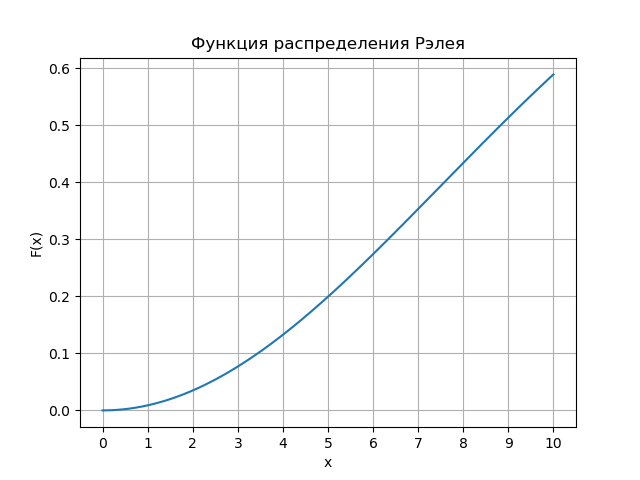
\includegraphics[width=\textwidth]{output/task2/rayleigh_chart.png}
\end{figure}

\begin{figure}[H]
\caption{График функции нормального распределения}
\includegraphics[width=\textwidth]{output/task2/norm_chart.png}
\end{figure}

\end{center}

\begin{table}[H]
\caption{Результаты}
\label{tab:my_label1}
\begin{center}
\vspace{5mm}
\begin{tabular}{|c|c|c|c|}
\hline
Распределение & $n$&Тест по критерию $\omega^2$ & Тест по критерию $\omega^2$ для нормального распределения \\
\hline
&$50$&	$True$&		$True$ \\
\cline{2-4}
&$200$&	$True$&		$True$ \\
\cline{2-4}
\raisebox{1.5ex}[0cm][0cm]{Фишер}&$1000$&	$True$&		$True$\\
\hline
&50&	$True$&		$True$ \\
\cline{2-4}
&$200$&	$False$&		$True$ \\
\cline{2-4}
\raisebox{1.5ex}[0cm][0cm]{Рэлея}&$1000$&	$True$&	$True$\\
\hline
\end{tabular}
\end{center}
\end{table}

\section{Выводы}

По полученным результатам видно, что оба подхода дают лучший результат на выборках большого объема. Если рассматривать результаты для выборки объема $n=200$ элементов, то видно, что при распределении Фишер тест на критерий Крамера — Мизеса — Смирнова пройден в отличии от Рэлея.

\begin{thebibliography}{}
    \bibitem{numpy}  Модуль numpy  -  https://physics.susu.ru/vorontsov/language/numpy.html
    
    \bibitem{plotlib} 
    Модуль matplotlib - https://matplotlib.org/users/index.html
    
    \bibitem{skp}
    Модуль scipy - https://docs.scipy.org/doc/scipy/reference/
    

\bibitem{8_1}
Большев Л.Н., Смирнов Н.В. Таблицы математической статистики. М.: Наука, 1983.

\bibitem{8_2}
http://www.machinelearning.ru/

\bibitem{8_3}
https://ru.wikipedia.org/

\end{thebibliography}

\section{Приложения}


Код отчёта:\; \url{https://github.com/9Shikamaru/CourseProjMatStat}

\end{document}
